\chapter{A Tight Bound on Grids of Size $\geq$ 5}

\section{Introduction and Definitions}
Let the ordered tuple $(a,b,c)$ represent the $a \times b \times c$ grid $G$ where $a \geq b \geq c$. We refer to $c$ as the ``thickness" of $G$. For example, the tuple $(5,3,3)$ represents a $5 \times 3 \times 3$ grid of thickness 3. We refer to a tuple as ``divisible", or a ``divisibility case", if and only if $ab+bc+ca \equiv 0 \pmod 3$. Observe that the divisibility cases are precisely those grids with integral lower bounds. The divisibility cases of thicknesses belonging to the three residue classes modulo 3 are illustrated in \{Figure something\}.

In the following lemmas, we use the notation $(a,b,c)+(x,y,z) = (a+x, b+y, c+z)$ to represent respective increases of $x$, $y$, and $z$ to the side lengths $a$, $b$, and $c$ of $G$. We note the following: 
\begin{rem}
\label{rem:recursion_pieces}
By applying the recursion, $(a,b,c)+(x,y,z)$ percolates at the lower bound when either:
\begin{enumerate}
\item $(a,b,c), (a,y,z), (x,b,z), (x,y,c)$ all percolate at the lower bound, or;
\item $(x,y,z), (x,b,c), (a,y,c), (a,b,z)$ all percolate at the lower bound.
\end{enumerate}
\end{rem}

We shall call a thickness ``complete" if it can be shown that all divisibility cases in that thickness percolate at the lower bound. In this section, we demonstrate that thickness 5, thickness 6 and thickness 7 are all complete. As these belong to the residue classes 2, 0, and 1 modulo 3, respectively, we then use a recursive construction to show that all larger grids are also complete. 

\section{Completeness of Thickness 5}
Leveraging \{lemmas from earlier chapters yet to be written\}, we show that all divisibility cases in thickness 5 percolate at the lower bound. 

NOTE: THE FOLLOWING LEMMAS HOLD ASSUMING WE HAVE A GENERAL CONSTRUCTION FOR $(2,3,3k)$ FOR ALL $k$.
\begin{lem}
\label{lem:width_5}
All divisibility cases for grids of the form $(k,5,5)$ percolate at the lower bound.
\end{lem}

\begin{proof}
We consider grids obtained from $(5,2,2) + (a,3,3)$, for $a \equiv 0 \pmod 3$ and $a >3$. By remark \ref{rem:recursion_pieces}, it is sufficient to show that $(5,2,2), (5,3,3), (a,2,3), (a,2,3)$ are all perfect. By \{a bunch of constructions\}, each of these grids percolates at the lower bound for $a>3$. We therefore obtain all grids of the form $(k,5,5)$, for $k>8$. The only missing grids are $(5,5,5)$ and $(8,5,5)$, which we have by construction. This completes the proof. 
\end{proof}

\begin{lem}
\label{lem:width_6}
All divisibility cases for grids of the form $(k,6,5)$ percolate at the lower bound.
\end{lem}

\begin{proof}
We consider grids obtained from $(6,3,2) + (a,3,3)$, for $a \equiv 0 \pmod 3$ and $a >3$. By remark \ref{rem:recursion_pieces}, it is sufficient to show that $(6,3,2), (6,3,3), (a,3,3), (a,3,2)$ are all perfect. By \{a bunch of constructions\}, each of these grids percolates at the lower bound for $a>3$. We therefore obtain all grids of the form $(k,6,5)$, for $k>8$. The only missing grid is $(6,6,5)$, which we have by construction. This completes the proof. 
\end{proof}

\begin{lem}
Thickness 5 is complete.
\end{lem}

\begin{proof}
Let $(a,b,2)$ represent an arbitrary (divisible) grid of thickness 2, and let $x = a \pmod 6$ and $y = b \pmod 6$. By \{some as of yet unwritten construction\}, we have that $(a,b,2)$ percolates at the lower bound for all $x,y \in \{0,2,3,5\}$, where $x \neq y$. We consider two constructions: $(a,b,2) + (6,3,3)$ and $(a,b,2) + (6,6,3)$. 

By item (1) of the remark, in order to show that $(a,b,2) + (6,3,3)$ percolates at the lower bound, it is sufficient to show that $(a,b,2), (a,3,3), (6,b,3), (6,3,2)$ all percolate at the bound. By \{more unwritten constructions\}, this is true for all $x,y \in \{0,2,3,5\}$, where $x \neq y$, $a,b > 1$, and at least one of $\{a,b\} > 2$. (Note that if $a=2$, one of the tuples is $(2,3,3)$, which does not percolate at the lower bound; we accommodate for this by re-writing $(a,b,2) + (6,3,3)$ as $(a,b,2) + (3,6,3)$.) The resulting tuple $(a', b', 5)$ is a grid of thickness 5, with $a'$ and $b'$ in the same residue class modulo $6$, $x,y \geq 8$, and at least one of $\{a',b'\} \geq 9$. From \{some figure representing the divisibility cases of thickness 5\}, we see that the lower bound on $a'$ and $b'$ omits all grids of the form $(5,5,k)$ and $(5,6,k)$, as well as the singular grid $(8,8,5)$. 

Applying an analogous argument to $(a,b,2) + (6,6,3)$, we must demonstrate that $(a,b,2), (a,6,3), (6,b,3), (6,6,2)$ all percolate at the lower bound. By \{some other constructions\}, we again find that this holds for all $x,y \in \{0,2,3,5\}$, where $x \neq y$ and $a,b > 1$. This gives all thickness 5 tuples $(a',b', 5)$ with $a'$ and $b'$ in different residue classes modulo $6$, where $a',b' \geq 8$. 

Combining these results, we have completeness for all grids of thickness 5 except those of the form $(5,5,k)$ and $(5,6,k)$. By lemmas \ref{lem:width_5} and \ref{lem:width_6}, these cases are also complete, and so thickness 5 is complete. This completes the proof. 
\end{proof}

\section{Completeness of Thickness 6}
We shall show that all grids of thickness 6 can be obtained recursively from $(3, 3n,m)$, where $n,m \equiv 1 \pmod 2$ (see construction \{something\}), and one of $\{(3,3,3), (6,3,3), (6,6,3)\}$. As the following proof requires examining a number of cases, we separate thickness 6 into three categories, and show that each of these categories is complete. 

\begin{figure}[]
\centering
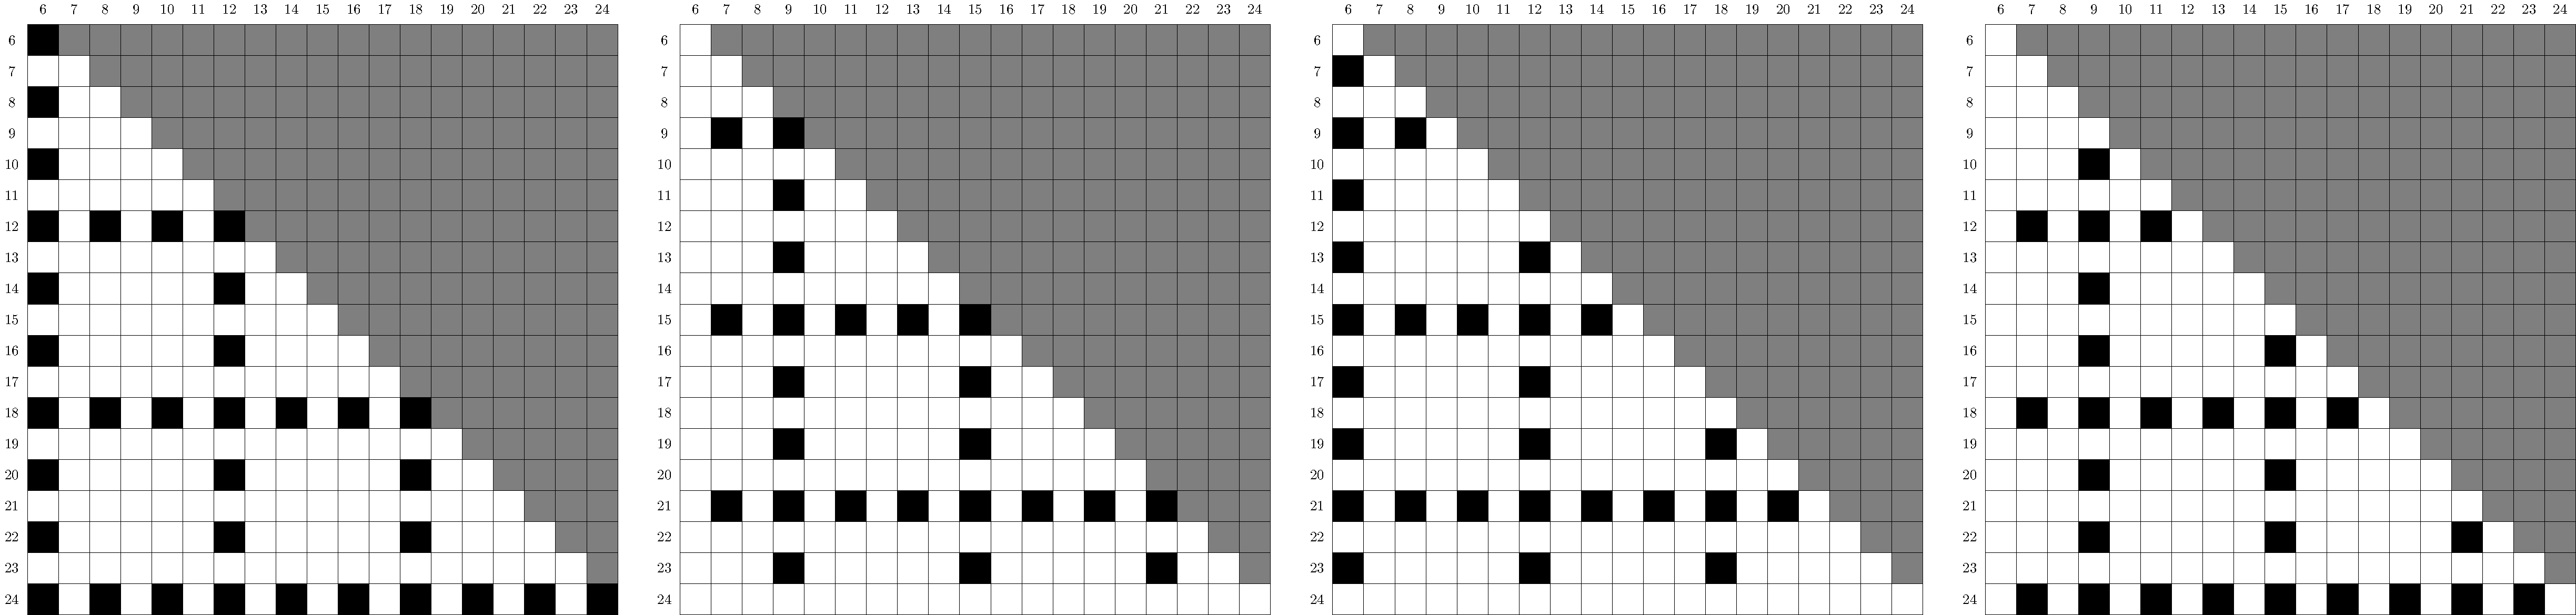
\includegraphics[width=\textwidth]{figures/3/thickness_6_case_1.pdf}
\caption{Thickness 6 grids with perfect percolating sets as obtained in lemma \ref{lem:thickness_6_case_1} (left), and divisibility cases of thickness 6 (right).}
\label{fig:thickness_6_case_1}
\end{figure}

\begin{lem}
\label{lem:thickness_6_case_1}
All grids of the form $(a,b,6)$, where $a \equiv 0 \pmod 6$ and $b \equiv 0 \pmod 2$, or $b \equiv 0 \pmod 6$ and $a \equiv 0 \pmod 2$, percolate at the lower bound.
\end{lem}

\begin{proof}
We consider $(3,3n,m) + (3,3,3)$, for $n,m \equiv 1 \pmod 2$. Observe that the resulting grid is of the form $(6, 3k, l)$, where $k,l \equiv 0 \pmod 2$. This, in turn, is precisely the set of grids described above. By remark \ref{rem:recursion_pieces}, we have that $(3,3n,m) + (3,3,3)$ percolates if $(3,3n,m), (3,3,3), (3,3n,3),(3,3,m)$ all percolate. By construction \{yet to be named\}, all grids $(a,3,3)$ are perfect. Therefore, $(3,3n,m) + (3,3,3)$ is perfect. This completes the proof.
\end{proof}

\begin{lem}
\label{lem:thickness_6_case_2}
All grids of the form $(a,b,6)$, where $a \equiv 3 \pmod 6$ and $b \equiv 1 \pmod 2$, or $b \equiv 3 \pmod 6$ and $a \equiv 1 \pmod 2$, percolate at the lower bound.
\end{lem}

\begin{proof}
Same argument as above, but add $(3,6,6)$. 
\end{proof}

\begin{lem}
\label{lem:thickness_6_case_3}
All remaining grids for thickness 6 work.
\end{lem}

\begin{proof}
Add $(3,6,3)$ or $(3,3,6)$.
\end{proof}

\begin{lem}
Thickness 6 is complete.
\end{lem}

\begin{proof}
Lemmas \ref{lem:thickness_6_case_1}, \ref{lem:thickness_6_case_2}, and \ref{lem:thickness_6_case_3} cover all divisibility cases for thickness 6. The result follows.
\end{proof}

\section{Completeness of Thickness 7}

We show that all divisibility cases for grids of thickness 7 percolate at the lower bound. Observe that divisibility cases for thickness 7 consist of grids of the form $(x,y,7)$ for $x,y$ in residue classes $\{0,1,3,4\}$ modulo 6. We separate these divisibility cases into the following four categories and show that each category is complete:
\begin{enumerate}
\item $(x,y,7)$ for $x,y \in \{1,4\}$ and $x \equiv y \pmod 6$;
\item $(x,y,7)$ for $x,y \in \{1,4\}$ and $x \not\equiv y \pmod 6$;
\item $(x,y,7)$ for $x,y \in \{0,3\}$ and $x \equiv y \pmod 6$;
\item $(x,y,7)$ for $x,y \in \{0,3\}$ and $x \not\equiv y \pmod 6$.
\end{enumerate}

\begin{lem}
\label{lem:thickness_7_case_1}
All grids of the form $(x,y,7)$ for $x,y \in \{1,4\}$ and $x \equiv y \pmod 6$ are complete.
\end{lem}

\begin{proof}
Consider the construction $(a,b,2) + (8,5,5)$ for $a,b \in \{2,5\}$ and $a \not\equiv b \pmod 6$. Observe that this construction obtains all grids of the form described in (1) above. We show that the grids $(a,b,2), (a,5,5), (8,b,5), (8,5,2)$ are all complete. \{The fact that these grids are complete follows from a number of constructions and the observation that thickness 5 is complete.\} By remark \ref{rem:recursion_pieces}, the construction $(a,b,2) + (8,5,5)$ percolates at the lower bound. This completes the proof. 
\end{proof}

\begin{lem}
\label{lem:thickness_7_case_2}
All grids of the form $(x,y,7)$ for $x,y \in \{1,4\}$ and $x \not\equiv y \pmod 6$ are complete.
\end{lem}

\begin{proof}
Consider the construction $(a,b,2) + (5,5,5)$ for $a,b \in \{2,5\}$ and $a \not\equiv b \pmod 6$. The same argument as above shows that this construction is perfect.
\end{proof}

\begin{lem}
\label{lem:thickness_7_case_3}
All grids of the form $(x,y,7)$ for $x,y \in \{0,3\}$ and $x \equiv y \pmod 6$ are complete.
\end{lem}

\begin{proof}
Consider the construction $(a,b,2) + (5,6,9)$ for $a,b \in \{0,3\}$ and $a \not\equiv b \pmod 6$. Same idea.
\end{proof}

\begin{lem}
\label{lem:thickness_7_case_4}
All grids of the form $(x,y,7)$ for $x,y \in \{0,3\}$ and $x \not\equiv y \pmod 6$ are complete.
\end{lem}

\begin{proof}
Consider the construction $(a,b,2) + (5,6,6)$ for $a,b \in \{0,3\}$ and $a \not\equiv b \pmod 6$. Same idea.
\end{proof}

\begin{lem}
Thickness 7 is complete.
\end{lem}

\begin{proof}
By lemmas \ref{lem:thickness_7_case_1}, \ref{lem:thickness_7_case_2}, \ref{lem:thickness_7_case_3}, and \ref{lem:thickness_7_case_4}, all divisibility cases for thickness 7 percolate at the lower bound.
\end{proof}

\section{Completeness of Grids of Size $\geq$ 5}

We can get completeness in every residue class modulo 3 by simply considering the grids obtained from $(x,y,z)+(3,3,3)$. TA-DA!




